\documentclass{beamer}
\usepackage{listings}
\usepackage{xcolor}
\usepackage{graphicx}
\usepackage{float}
\usepackage{tikz}
\usetikzlibrary{trees}
\usepackage{hyperref}
\usepackage{array}

\setbeamertemplate{navigation symbols}{}

\hypersetup{
    colorlinks=true,
    linkcolor=blue,
    filecolor=magenta,
    urlcolor=blue
}

\urlstyle{same}

\title{Bash Workshop I: The Basics}
\author{Frederick Yin}
\institute{JITech}
\date{2023}

\definecolor{codegreen}{rgb}{0,0.6,0}
\definecolor{codegray}{rgb}{0.5,0.5,0.5}
\definecolor{codepurple}{rgb}{0.58,0,0.82}
\definecolor{backcolour}{rgb}{0.95,0.95,0.92}

\lstdefinestyle{wksp}{
    backgroundcolor=\color{backcolour},
    commentstyle=\color{codegreen},
    keywordstyle=\color{magenta},
    numberstyle=\tiny\color{codegray},
    stringstyle=\color{codepurple},
    basicstyle=\ttfamily\footnotesize,
    breakatwhitespace=false,
    breaklines=true,
    captionpos=b,
    keepspaces=true,
    numbers=left,
    numbersep=5pt,
    showspaces=false,
    showstringspaces=false,
    showtabs=false,
    tabsize=4
}

\lstset{style=wksp}

\graphicspath{{./img/}}

\AtBeginSection[]{
    \begin{frame}
        \frametitle{Table of Contents}
        \tableofcontents[currentsection]
    \end{frame}
}

\renewcommand{\tt}{\texttt}

\begin{document}
\frame{\titlepage}

% !TeX root = bash.tex
\section{Intro}
\begin{frame}
\frametitle{A brief history of bash}
\begin{figure}[h]
    \centering
    
\includegraphics[height=3cm]{bash_logo}
\end{figure}
\begin{itemize}
    \item Born: 1989
    \item Probably played Pokémon on the Game Boy
    \item Is an umbrella term for zsh, fish, …
    \item Runs on Unix-like environments
\end{itemize}
\end{frame}

\begin{frame}
\frametitle{A brief history of Unix}
\begin{itemize}
    \item Born: 1969
    \item Probably listened to Michael Jackson
    \item Gave rise to Linux, BSD, and Mac OS
    \item We call them ``Unix-like''
\end{itemize}
\end{frame}

\begin{frame}
\frametitle{Unix: The Good Part}
The Unix philosophy (paraphrased):
\begin{itemize}
    \item Store data in plain text
    \item Hierarchical file system
    \item Everything is a file
    \item One tool does one thing
    \item Tools together strong
\end{itemize}
\begin{block}{Quote}
The power of a system comes more from the relationships among programs than
from the programs themselves.
\begin{flushright}
    — Brian Kernighan and Rob Pike
    \footnote{The UNIX Programming Environment. 1984. viii}
\end{flushright}
\end{block}
\end{frame}

\begin{frame}
\frametitle{Unix: The Chaotic Part}
``Unix'' is mostly created by these three groups of people who routinely
disagree with each other:\footnote{Not convinced? Try \tt{man ps}.}
\begin{figure}[h]
    \centering
    
\includegraphics[height=3cm]{gnu_linux_bsd}
    \caption{GNU, Linux, and BSD\footnote{Yes, I know there are many BSDs}}
\end{figure}
Despite this, they all hate Microsoft.

We will be talking about GNU today.
\end{frame}

\begin{frame}
\frametitle{Before we start}
\begin{itemize}
    \item This is \textbf{not} a Linux workshop
        (although I encourage you to use it)
    \item This is not a vim workshop either
    \item You should use a \tt{monospace} font
    \item Anyone caught using PowerShell will be kicked out of the venue
\end{itemize}
\end{frame}

\begin{frame}[fragile]
\frametitle{Conventions in slides}
\begin{itemize}
    \item \tt{\$} indicates a \textbf{bash command}.
        Do not type the \tt{\$}.
    \item \tt{\#} indicates a \textbf{comment}.
        Do not type it or anything after it.
\end{itemize}
For example, when you see:
\begin{lstlisting}[language=bash]
$ echo hello  # printf("hello\n");
\end{lstlisting}
You are going to type:
\begin{lstlisting}[language=bash]
echo hello
\end{lstlisting}
I encourage you to type commands by hand.
\end{frame}

% !TeX root = bash.tex
\section{I. Files \& File Tree}
\begin{frame}[fragile]
\frametitle{Files}
Each of these is a different \textbf{file}:
\begin{itemize}
    \item \tt{a}
    \item \tt{.a} (Hidden)
    \item \tt{a.txt}
    \item \tt{A.txt}
    \item \tt{A.TXT}
\end{itemize}

\begin{block}{Note}
    The dot and suffix are part of the filename.
\end{block}

\begin{block}{Tip}
    For convenience, \textbf{avoid spaces} and most of the special characters
    (except \verb|._-|) when working in bash. If you have to, surround filename
    in quotes: \tt{`Lab Report (3) final FINAL-1.docx'}
\end{block}
\end{frame}

\begin{frame}[fragile]
    \frametitle{\tt{cat}: Printing a file}
Try this inside \tt{01-files/}:
\begin{lstlisting}[language=bash]
$ cat a
$ cat .a
$ cat a.txt
\end{lstlisting}
\begin{block}{Explanation}
    \tt{cat} is short for ``concatenate'' (to join together) but it's
    mostly used to print files.
\end{block}
\end{frame}

\begin{frame}[fragile]
\frametitle{\tt{cp, mv, rm}: Relocating a file}
Try this inside \tt{01-files/}:
\begin{lstlisting}[language=bash]
$ cp a b
$ mv a.txt b.txt
$ rm b
\end{lstlisting}
\begin{block}{Explanation}
    \begin{itemize}
        \item ``copy'' \tt{a} into a file called \tt{b}
        \item ``move'' \tt{a.txt} into a file called \tt{b.txt}
        \item ``remove'' \tt{b}
    \end{itemize}
\end{block}
\end{frame}

\begin{frame}[fragile]
\frametitle{\tt{cp, mv}: Overwriting and renaming}
When the destination does not exist, \tt{cp} and \tt{mv} simply create
that file. \textbf{Otherwise, it is destroyed and overwritten.}
\newline \newline
Try this inside \tt{01-files/}:
\begin{lstlisting}[language=bash]
$ cp a b      # b is created
$ cp a a.txt  # a.txt is overwritten
\end{lstlisting}

When you \tt{mv} a file into a file that doesn't exist, you are essentially
\textbf{renaming} it. Recall this command from last slide:
\begin{lstlisting}[language=bash]
$ mv a.txt b.txt
\end{lstlisting}
\end{frame}

\begin{frame}
\frametitle{Directories}
Each of these is a \textbf{directory} (``dir'' for short):
\begin{itemize}
    \item \tt{dir/}
    \item \tt{01-files/}
    \item \tt{01-files/dir/}
    \item \tt{01-files/.dir/} (Hidden dir)
\end{itemize}

\begin{block}{Convention}
    For clarity, we add a slash (\tt{/}) to the end of a directory in the
    slides.    However, in reality it often makes no difference.
\end{block}
\end{frame}

\begin{frame}[fragile]
\frametitle{\tt{cd, pwd}: Changing directory}
Try this inside \tt{01-files/}:
\begin{lstlisting}[language=bash]
$ cd dir/
$ pwd
$ cd ../
$ pwd
\end{lstlisting}
\begin{block}{Explanation}
    \begin{itemize}
        \item \tt{cd} is short for ``change directory''
        \item \tt{pwd} is short for ``print working directory''
        \item \tt{..} is a special directory. It is the ``parent''
    \end{itemize}
\end{block}
\end{frame}

\begin{frame}[fragile]
\frametitle{\tt{ls}: Listing directories}
Try this inside \tt{01-files/}:
\begin{lstlisting}[language=bash]
$ ls
$ ls -a
$ ls -l
$ ls -a -l
$ ls dir/
\end{lstlisting}
\begin{block}{Explanation}
    \begin{itemize}
        \item \tt{ls} is short for ``list''
        \item \tt{-a} is short for \tt{--all}
        \item \tt{-l} enables long listing format
    \end{itemize}
\end{block}
\end{frame}

\begin{frame}[fragile]
\frametitle{\tt{mkdir, rm}: Creating and deleting directories}
Try this inside \tt{01-files/}:
\begin{lstlisting}[language=bash]
$ mkdir dir/
$ rm -r dir/
$ mkdir -p dir/subdir/
$ ls dir/
\end{lstlisting}
\begin{block}{Explanation}
    \begin{itemize}
        \item \tt{mkdir} stands for ``make directory''
        \item \tt{-r} is short for \tt{--recursive}
        \item \tt{-p} is short for \tt{--parents}
    \end{itemize}
\end{block}
\end{frame}

\begin{frame}[fragile]
\frametitle{\tt{cp, mv}: Into and out of directories}
Try this inside \tt{01-files/}:
\begin{lstlisting}[language=bash]
$ cp a dir/
$ mv b.txt dir/
$ mv b.txt dir/a
$ mv dir/a b.txt
\end{lstlisting}
\begin{block}{Explanation}
    \begin{itemize}
        \item Line 1 copies \tt{a} into \tt{dir/}
        \item Line 2 moves \tt{b.txt} into \tt{dir/}
        \item Line 3 moves \tt{b.txt} into \tt{dir/} and overwrite
            \tt{dir/a}
        \item Line 4 moves \tt{dir/a} back into \tt{b.txt}
    \end{itemize}
\end{block}
\end{frame}

\begin{frame}
\frametitle{File tree}
Think of any directory as a tree.

\begin{figure}[h]
    \centering
    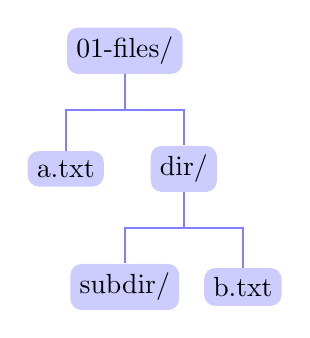
\begin{tikzpicture}
        \tikzstyle{every node}=[fill=blue!20,rounded corners]
        \tikzstyle{edge from parent}=[blue!50,thick,draw]
        \node {01-files/}[edge from parent fork down]
            child {node {a.txt}}
            child {
                node {dir/}
                    child {node {subdir/}}
                    child {node {b.txt}}
            };
    \end{tikzpicture}
\end{figure}
\end{frame}

\begin{frame}
\frametitle{Paths}
File $\cup$ directory = \textbf{path}.
\footnote{At least in the scope of this workshop.}
\newline \newline

No paths under the same directory can bear the same name.
These \textbf{cannot} coexist:
\begin{itemize}
    \item \tt{01-files/data/}, a directory
    \item \tt{01-files/data}, a regular file
\end{itemize}
\end{frame}

\begin{frame}
\frametitle{Absolute \& relative paths}
\begin{itemize}
    \item Paths beginning with \tt{/} are absolute: \tt{/usr/bin/cat}
    \item Otherwise it is relative: \tt{01-files/}
\end{itemize}

If you know where you are, you can convert a relative path to an absolute one.
\begin{example}
    Your location: \tt{/home/you/} \newline
    Relative path: \tt{bash-workshop/01-files/} \newline
    Absolute path: \tt{/home/you/bash-workshop/01-files/}
\end{example}
\end{frame}

\begin{frame}
\frametitle{Wildcard}
\tt{*} is a character to match any number of (including zero) characters.

\begin{block}{Exception}
    Hidden paths will remain hidden unless you explicitly specify the dot:
    \tt{.*}
\end{block}

\begin{example}
    Consider a dir containing \tt{a/}, \tt{b/}, \tt{a-copy.txt} and
    \tt{b.txt}.
    \begin{itemize}
        \item \tt{*} matches \tt{a/ b/ a-copy.txt b.txt}
        \item \tt{a*} matches \tt{a/ a-copy.txt}
        \item \tt{*.txt} matches \tt{a-copy.txt b.txt}
    \end{itemize}
\end{example}

\scriptsize{Technically it's called a glob pattern but who cares. Also there are other
weird symbols like \tt{?} or \tt{[]} but I swear \tt{*} is most of
us will ever use.}
\end{frame}

\begin{frame}
\frametitle{\tt{.} and \tt{..}}
Inside every dir\footnote{Except \tt{/}} there are two special dirs:
\begin{itemize}
    \item \tt{.} — current dir
    \item \tt{..} — parent dir
\end{itemize}

You can use them in relative paths.
\begin{example}
    Your location: \tt{/home/you/} \newline
    Relative path: \tt{../friend/bash-workshop/01-files/} \newline
    (Note that \tt{/home/you/../friend/} is just \tt{/home/friend/}) \newline
    Absolute path: \tt{/home/friend/bash-workshop/01-files/}
\end{example}
\end{frame}

\begin{frame}<presentation:0>[fragile]
\frametitle{Quiz: Expand relative paths}
Suppose your home directory is \tt{/home/sjtu/} and you are currently in
\tt{/home/sjtu/lbl/}. Expand these relative paths to absolute ones:
\begin{itemize}
    \item \tt{lobby}
    \item \tt{3f/ylm}
    \item \tt{./elevator}
    \item \tt{../library/}
    \item \tt{../../fdu/}
    \item \verb|~/lawson| % \tt doesn't format ~ well
\end{itemize}
\end{frame}

\begin{frame}<presentation:0> % hide frame
\frametitle{Answer}
\begin{itemize}
    \item \tt{/home/sjtu/lbl/lobby}
    \item \tt{/home/sjtu/lbl/3f/ylm}
    \item \tt{/home/sjtu/lbl/elevator}
    \item \tt{/home/sjtu/library/}
    \item \tt{/home/fdu/}
    \item \tt{/home/sjtu/lawson}
\end{itemize}
\end{frame}

\begin{frame}<presentation:0>
\frametitle{File commands cheatsheet (part 1)}
% TODO pwd
\begin{itemize}
    \item \tt{cat FILE} — print out FILE
    \item \tt{cd DIR/} — change current directory to DIR
    \begin{itemize}
        \item \tt{cd} — go to home dir
    \end{itemize}
    \item \tt{ls DIR/} — list dirs and files in DIR
    \begin{itemize}
        \item \tt{ls} — list current dir
    \end{itemize}
    \item \tt{pwd} — print where you are
    \item \tt{mkdir DIR/} — create dir named DIR
    \item \tt{rm FILE} — remove FILE
    \begin{itemize}
        \item \tt{rm -r DIR/} — remove everything in DIR and itself
        \item \tt{rm -r DIR/*} — remove everything in DIR but not DIR
    \end{itemize}
\end{itemize}
\end{frame}

\begin{frame}<presentation:0>
\frametitle{File commands cheatsheet (part 2)}
\begin{itemize}
    \item \tt{cp SRC DEST} — copy file named SRC to DEST
    \begin{itemize}
        \item \tt{cp SRC DEST\_DIR/} — copy SRC into DEST\_DIR/
        \item \tt{cp -r SRC\_DIR/ DEST\_DIR/}
            — copy SRC\_DIR/ and everything inside into DEST\_DIR
    \end{itemize}
    \item \tt{mv SRC DEST} — move (rename) SRC to DEST
    \begin{itemize}
        \item \tt{mv SRC DEST\_DIR/} — move SRC into DEST\_DIR
        \item \tt{mv SRC\_DIR/ DEST\_DIR/}
            — move SRC\_DIR into DEST\_DIR (no \tt{-r} needed)
    \end{itemize}
\end{itemize}
\begin{alertblock}{Warning}
    \tt{cp} and \tt{mv} will overwrite your files by default.
    How to avoid that? Check your cheatsheet.
\end{alertblock}
\end{frame}

\begin{frame}
\frametitle{Task}
Inside \tt{01-files/}:
\begin{itemize}
    \item Enter \tt{task/}
    \item Create \tt{backup/}
    \item Copy \tt{a.txt} into \tt{dir/}
    \item Move \tt{dir/} into \tt{backup/}
    \item Verify if you succeeded using \tt{ls}
    \item Delete \tt{backup/}
\end{itemize}
\end{frame}

\begin{frame}<presentation:0>[fragile]
\frametitle{Solution}
\begin{lstlisting}[language=bash]
$ mkdir backup/
$ cp a.txt dir/
$ mv dir/ backup/
$ ls
# Output: backup/  a.txt
$ ls backup/dir/
# Output: a.txt
$ rm -r backup/
\end{lstlisting}
\end{frame}

% !TeX root = bash.tex
\section{II. CLI}
\begin{frame}
\frametitle{The CLI}
\textbf{CLI} stands for \textbf{command line interface}, as opposed to a GUI.

\begin{figure}[h]
    \centering
    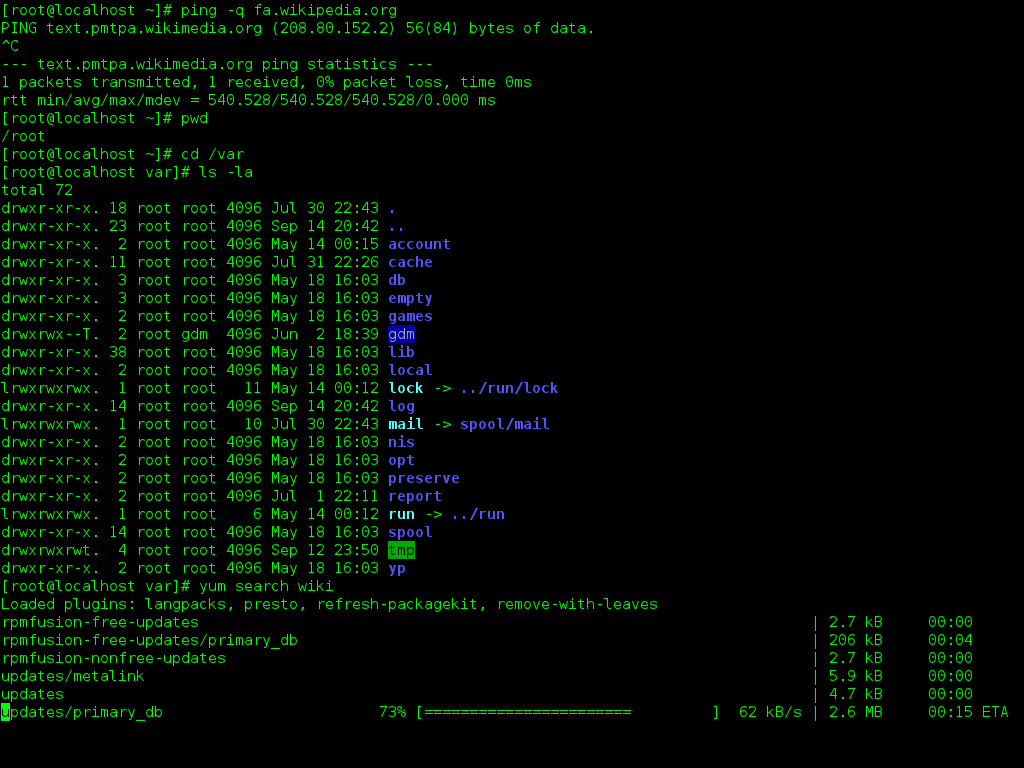
\includegraphics[height=5cm]{cli}
    \caption{A stereotypical, Hollywood-like CLI.}
\end{figure}
\end{frame}

\begin{frame}[fragile]
\frametitle{Anatomy of a command}
\begin{lstlisting}[language=bash]
# get first 5 lines of file
$ head -n 5 longfile.txt
\end{lstlisting}
\begin{tabular}{ll}
    \tt{head}            & Executable file somewhere \\
    \tt{-n}              & Option (aka flag) \\
    \tt{5}               & Argument to \tt{-n} \\
    \tt{longfile.txt}    & Argument to \tt{head}
\end{tabular}
\end{frame}

\begin{frame}[fragile]
\frametitle{Anatomy of a command}
Anatomy of a command:
\begin{lstlisting}[language=bash]
# list all files but *.o recursively in reverse
$ ls -Rr --ignore='*.o'
\end{lstlisting}
\begin{tabular}{ll}
    \tt{ls}             & Executable in \tt{\$PATH} \\
    \tt{-Rr}            & Two options: \tt{-R -r} \\
    \tt{--ignore=}      & Long option \\
    \tt{'*.o'}          & Argument to \tt{--ignore}
\end{tabular}
\begin{block}{Notes}
    \begin{itemize}
        \item Not every program uses this \tt{--long-option} convention
        \item The equal sign after \tt{--ignore} is optional in this command
        \item \tt{'*.o'} does \textit{not} expand to a list of files.
            It is simply a string.
    \end{itemize}
\end{block}
\end{frame}

\begin{frame}[fragile]
\frametitle{I can't possibly remember all \tt{--this} and \tt{--that}!}
You don't need to, thanks to \textbf{man pages}! (Short for manual pages)
\newline \newline
Try:
\begin{lstlisting}[language=bash]
$ man ls
\end{lstlisting}

If it doesn't work, try \url{https://man.archlinux.org/man/ls.1}
\end{frame}

\begin{frame}[fragile]
\frametitle{Challenge}
\begin{itemize}
    \item Read the man page for \tt{head}
    \item Experiment with files in \tt{02-cli/}
    \item Find a command to generate the following:
\end{itemize}
\begin{lstlisting}[language=bash]
==> p0.txt <==
MANIFESTO OF THE COMMUNIST PARTY.

==> p1.txt <==
I. BOURGEOIS AND PROLETARIANS.
\end{lstlisting}
\end{frame}

\begin{frame}<presentation:0>[fragile]
\frametitle{Solution}
\begin{lstlisting}[language=bash]
$ head -n1 -v p0.txt p1.txt
\end{lstlisting}
\end{frame}

\begin{frame}[fragile]
\frametitle{Learning by doing}
Inside \tt{02-cli/}, run:
\begin{lstlisting}[language=bash]
$ diff sway.1.conf sway.2.conf
\end{lstlisting}
Congratulations, you just learned how to use \tt{diff}!
\newline \newline
Now, what does this command do?
\begin{lstlisting}[language=bash]
$ comm -12 sway.1.conf sway.2.conf
\end{lstlisting}
\end{frame}

\begin{frame}
\frametitle{Lifehacks\footnote{Should work in most shells.}}
\begin{itemize}
    \item Use $\uparrow \downarrow$
    \item \tt{Ctrl-W}: delete one word to the left
    \item \tt{Ctrl-U}: delete everything to the left
    \item \tt{Ctrl-K}: delete everything to the right
    \item \tt{Ctrl-7}: undo
    \item \tt{Ctrl-C}: abort
    \item \tt{Ctrl-R}: search history
\end{itemize}
\end{frame}

% !TeX root = bash.tex
\section{III. Pipes}
\begin{frame}
\frametitle{stdout}
When you \tt{printf}, where does the string go?
\newline \newline
Your screen? Yes but also no.
\newline \newline
\tt{stdout}, or \textbf{standard output}, is a special file where \tt{printf}
dumps its output.\footnote{Yes, there's \tt{stderr} too, but we won't be talking
about it.}
\end{frame}

\begin{frame}[fragile]
\frametitle{Capturing stdout}
You can capture the stdout of a command and direct it somewhere else than your
screen, such as a file.
Try this:
\begin{lstlisting}[language=bash]
$ echo hello        # print to terminal
$ echo hello > out  # write to file
\end{lstlisting}
\begin{figure}
    \centering
    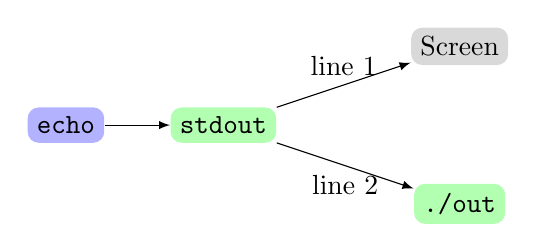
\begin{tikzpicture}
        \tikzstyle{every node}=[rounded corners]
        \node[fill=blue!30]  (prog)        at (0,  0) {\tt{echo}};
        \node[fill=green!30] (stdout)      at (2,  0) {\tt{stdout}};
        \node[fill=gray!30]  (term)        at (5,  1) {Screen};
        \node[fill=green!30] (stdout-file) at (5, -1) {\tt{./out}};
        \tikzstyle{every node}=[fill=none]
        \draw[-latex] (prog) -- (stdout);
        \draw[-latex] (stdout) -- (term) node[above,midway] {line 1};
        \draw[-latex] (stdout) -- (stdout-file) node[below,midway] {line 2};
    \end{tikzpicture}
\end{figure}
\end{frame}

\begin{frame}[fragile]
\frametitle{\tt{>} and \tt{>>}}
Try \tt{>>} instead of \tt{>}. What happens?
\begin{lstlisting}[language=bash]
$ echo hello >> out
$ cat out
\end{lstlisting}
Repeat a few times with both \tt{>} and \tt{>>}. What's the difference?
\pause
\begin{block}{Observation}
    \tt{>} overwrites the file, but \tt{>>} appends to it.
\end{block}
\end{frame}

\begin{frame}[fragile]
\frametitle{stdin}
The opposite of \tt{stdout} is \tt{stdin}: standard input.
Some programs read from stdin when they expect a path but aren't given any.
\newline \newline
Try this in \tt{03-pipes/}:
\begin{lstlisting}[language=bash]
$ ls random/ | head -n 5
\end{lstlisting}
\pause
\begin{block}{Observation}
    Normally \tt{head} expects a filename, but when none is given, it
    falls back to stdin — which is what \tt{ls} printed to stdout.
\end{block}
\begin{block}{Convention}
    We sometimes call the vertical bar (\tt{|}) the \textbf{pipe} character.
\end{block}
\end{frame}

\begin{frame}[fragile]
\frametitle{The power of pipes}
You can chain commands with pipes. Classic recipe (still in \tt{03-pipes}):
\begin{lstlisting}[language=bash]
$ cat numbers
$ cat numbers | sort
$ cat numbers | sort | uniq
$ cat numbers | sort | uniq | wc
\end{lstlisting}
\pause
\begin{block}{Observations}
    \begin{itemize}
        \item Each program takes the last one's stdout as stdin
        \item Only the final program will print to terminal
    \end{itemize}
\end{block}
\begin{block}{Explanation}
    \begin{itemize}
        \item By default, \tt{sort} sorts stdin in dictionary order
            (check man page for more)
        \item \tt{wc} is short for ``word count'', although the first thing
            it prints is the number of lines.
    \end{itemize}
\end{block}
\end{frame}

\begin{frame}[fragile]
\frametitle{Pipes illustrated}
\begin{lstlisting}[language=bash]
$ cat numbers | sort | uniq | wc
\end{lstlisting}
\begin{figure}
    \centering
    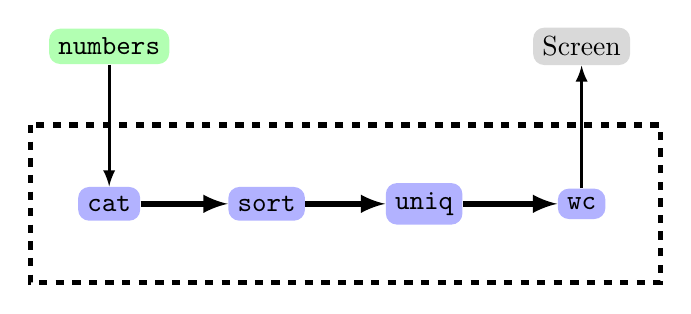
\begin{tikzpicture}
        \tikzstyle{every node}=[fill=blue!30, rounded corners]
        \node[fill=green!30] (numbers) at (-2, 2) {\tt{numbers}};
        \node (cat)         at (-2, 0) {\tt{cat}};
        \node (sort)        at (0,  0) {\tt{sort}};
        \node (uniq)        at (2,  0) {\tt{uniq}};
        \node (wc)          at (4,  0) {\tt{wc}};
        \node[fill=gray!30] (term) at (4,  2) {Screen};
        \tikzstyle{every node}=[fill=none]
        \tikzstyle{every path}=[-latex,line width=2pt]
        \draw[line width=1pt] (numbers) -- (cat);
        \draw (cat) -- (sort);
        \draw (sort) -- (uniq);
        \draw (uniq) -- (wc);
        \draw[line width=1pt] (wc) -- (term);
        \draw[dashed] (-3, 1) rectangle (5, -1);
    \end{tikzpicture}
\end{figure}
\begin{block}{Challenge}
    Can you think of a way to eliminate a pipe? (Hint: man sort)
    % sort numbers | uniq | wc
\end{block}
\end{frame}

\begin{frame}[fragile]
\frametitle{grep}
Try this in \tt{03-pipes}:
\begin{lstlisting}[language=bash]
$ ls random/ | grep JI
\end{lstlisting}
\pause
\begin{block}{Explanation}
    \tt{grep} is a powerful tool to match a substring. By default, it takes
    a file (or stdin), and prints all lines containing a pattern (``JI'').
\end{block}
\end{frame}

\begin{frame}
\frametitle{Challenge}
Inside \tt{03-pipes/random/}:
\begin{itemize}
    \item List all filenames containing ``FDU''
    \item List all filenames containing ``UM'' (upper and lower cases)
        (Hint: man grep)
    \item List all filenames containing ``UM'' but not ``FDU''
        (upper and lower cases for both substrings)
\end{itemize}
\end{frame}

\begin{frame}[fragile]
\frametitle{Solution}
\begin{lstlisting}[language=bash]
$ ls | grep FDU
$ ls | grep -i UM
$ ls | grep -i UM | grep -i -v FDU
\end{lstlisting}
\end{frame}

\begin{frame}
\frametitle{Conclusion}
\begin{itemize}
    \item Files and directories form a tree
    \item One tool does one thing, but flags specify how
    \item When in doubt, read documentation
    \item Chain together tools and unleash immense power
\end{itemize}
\end{frame}


\begin{frame}
\frametitle{The End}
\vspace{1cm}
\centering \Huge {Thank You For Coming!}
\end{frame}

\begin{frame}
\frametitle{Credits}
\begin{itemize}
    \item The Free Software Foundation, logo of GNU Bash.
        \url{https://commons.wikimedia.org/wiki/File:Gnu-bash-logo.svg}
    \item The Free Software Foundation, logo of GNU.
        \url{https://commons.wikimedia.org/wiki/File:The_GNU_logo.png}
    \item Larry Ewing, logo of Linux.
        \url{https://commons.wikimedia.org/wiki/File:Linux_logo.jpg}
    \item Poul-Henning Kamp, Beastie.
        \url{https://commons.wikimedia.org/wiki/File:Daemon-phk.svg}
    \item WikiMedia user ZxxZxxZ. Linux command-line.
        \url{https://commons.wikimedia.org/wiki/File:Linux_command-line._Bash._GNOME_Terminal._screenshot.png}
\end{itemize}
\end{frame}
\end{document}
